\documentclass[crop,tikz,convert={outext=.svg,command=\unexpanded{pdf2svg \infile\space\outfile}},multi=false]{standalone}[2012/04/13]

\usepackage[utf8]{inputenc}
\usepackage{amsmath, amssymb}
\usepackage{pgfplots}


%-------------------------------------
% Tikz and pgf options & definitions
%-------------------------------------
\pgfplotsset{compat=1.15}
\pgfmathsetseed{1}

\usetikzlibrary{positioning}
\usetikzlibrary{shapes}
\usetikzlibrary{backgrounds, fit}
\usetikzlibrary{calc}
\usetikzlibrary{decorations.markings}
\usetikzlibrary{matrix}

\def\colorvector at (#1,#2,#3){
\coordinate (A) at (#1, #2);
\filldraw[draw=black,fill=test!!+] (A)++(0,0) rectangle ++(0.25,0.25) node (A0) {};
\filldraw[draw=black,fill=test!!+] (A)++(0.3,0) rectangle ++(0.25,0.25) node (A1) {};
\filldraw[draw=black,fill=test!!+] (A)++(0.6,0) rectangle ++(0.25,0.25) node (A2) {};
\node[right=of A2, xshift=-7.5ex, yshift=-0.75ex] {$\ldots$};
\filldraw[draw=black,fill=test!!+] (A)++(1.5,0) rectangle ++(0.25,0.25) node (A4) {};
\node[left=of A1, xshift=4.4ex, yshift=-0.75ex] (BEG\i) {$#3=[$};
\node[right=of A4, xshift=-8ex, yshift=-0.75ex] (END\i) {$]^{T}$};
}

\begin{document}
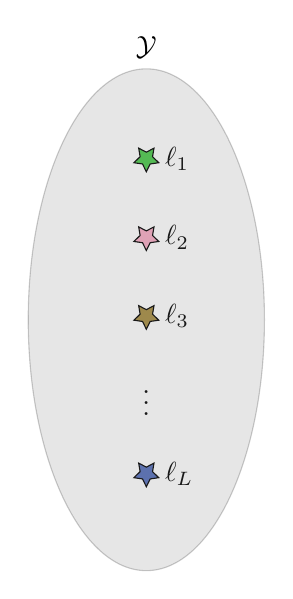
\begin{tikzpicture}[
    se/.style={draw,star,star points=5,star point ratio=0.5,fill=test!!++, minimum size=0.1cm}
    ]
\definecolorseries{test}{rgb}{step}[rgb]{.95,.85,.55}{.17,.47,.37}
\resetcolorseries[35]{test}
\node[se, label=right:$\ell_{1}$] at (0, 0) (LBL1) {};
\node[se, label=right:$\ell_{2}$] at (0, -1) (LBL2) {};
\node[se, label=right:$\ell_{3}$] at (0, -2) (LBL3) {};
\node[label=center:$\vdots$] at (0, -3) {};
\node[se, label=right:$\ell_{L}$] at (0, -4) (LBLL) {};
\node[fit={(LBL1)(LBLL)},draw, ellipse, fill=gray, opacity = 0.2, minimum width=3cm,minimum height=5cm,label=above:{${\cal Y	}$}](left){};    
\end{tikzpicture}
\end{document}